%%%%%%%%%%%%%%%%%%%%%%%%%%%%%%%%%%%%%%%%%%%%%%%%%%%%
% LECTURE 16
%%%%%%%%%%%%%%%%%%%%%%%%%%%%%%%%%%%%%%%%%%%%%%%%%%%%


%%
%%%%%%%%%%%%%%%%%%%%%%%%%%%%%%%%%%%%%%%%%%%%%%%%%%%%
\section*{Internal Flow Heat Transfer}
\addcontentsline{toc}{section}{Internal Flow Heat Transfer}
%%%%%%%%%%%%%%%%%%%%%%%%%%%%%%%%%%%%%%%%%%%%%%%%%%%%
Internal flows differ fundamentally from external flows in several important ways:

\begin{table}[h]
\centering
\begin{tabular}{|p{7cm}|p{7cm}|}
\hline
\textbf{External Flow} & \textbf{Internal Flow} \\
\hline
Heat transfer between surface and free-stream temperature $T_\infty$ & Heat transfer between surface and local bulk temperature (varying temperature)\\
\hline
Boundary layer grows continuously & Boundary layers grow until they meet, becoming fully developed \\
\hline
$\text{Re}_x$ varies with position along surface & $\text{Re}_D$ is constant throughout the flow \\
\hline
changing $\operatorname{Re}_{x,c}$ lead to different types of flows & Same flow type for all $\operatorname{Re}_{D,c}$ at different $x$\\
\hline
$h_x = q''_x/(T_s - \textcolor{red}{T_\infty})$ & $h_x = q''_x/(T_s - \textcolor{red}{T_m})$ 
\\
\hline
\end{tabular}
\end{table}
%
\begin{figure}[H]
    \centering
    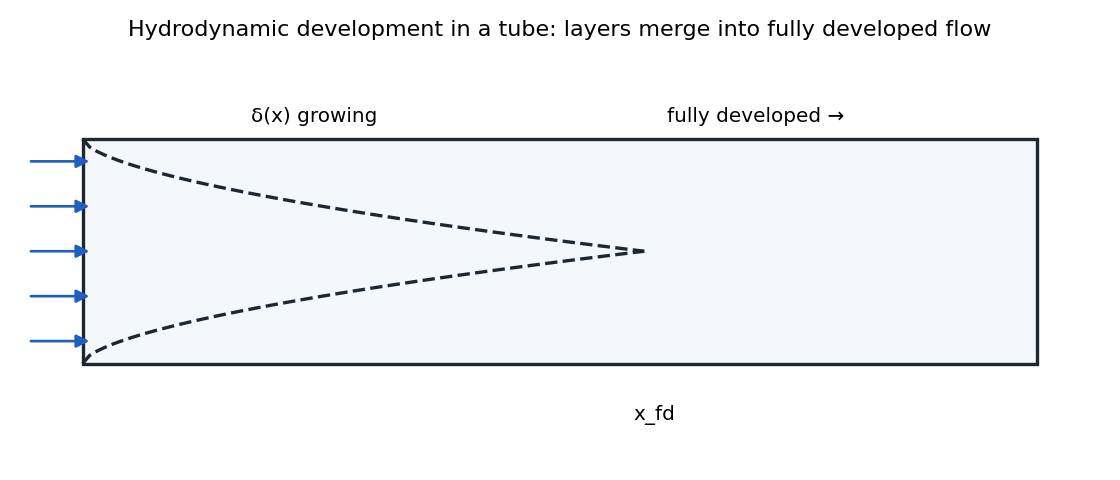
\includegraphics[width=0.80\linewidth]{pics/velocity_BL_in_pipe.png}
    \caption{Laminar, hydrodynamic boundary layer development in a circular tube.}
\end{figure}
%

%
For internal flows, the boundary layer development creates distinct flow regions:
\begin{itemize}
    \item Hydrodynamic entrance region (developing velocity profile)
    \item Hydrodynamic fully developed region (constant velocity profile)
\end{itemize}
%
\begin{figure}[H]
    \centering
    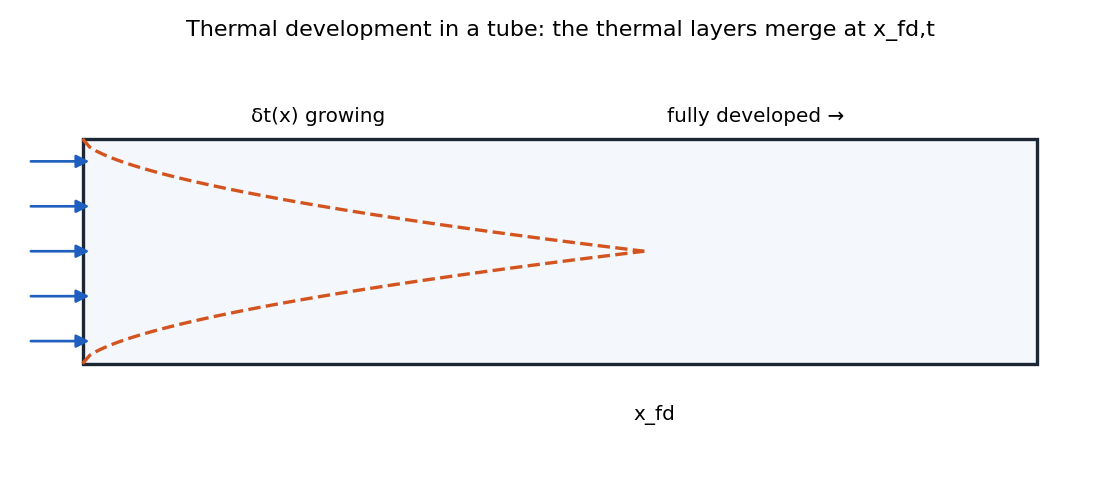
\includegraphics[width=0.80\linewidth]{pics/thermal_BL_in_pipe.png}
    \caption{Thermal boundary layer development in a circular tube.}
\end{figure}
%
Similarly for thermal boundary layers
%
\begin{itemize}
    \item Thermal entrance region (developing temperature profile)
    \item Thermally fully developed region (constant shape temperature profile)
\end{itemize}
%
%%%%%%%%%%%%%%%%%%%%%%%%%%%%%%%%%%%%%%%%%%%%%%%%%%%%%%%%%%%%
\subsubsection*{Internal Flow Concepts for Pipe Flow}
\addcontentsline{toc}{subsubsection}{Internal Flow Concepts for Pipe Flow}
%%%%%%%%%%%%%%%%%%%%%%%%%%%%%%%%%%%%%%%%%%%%%%%%%%%%%%%%%%%%
When fluid enters a pipe, boundary layers develop along the walls. Eventually, these boundary layers meet at the centerline, and the flow becomes fully developed.

The critical Reynolds number for circular pipe flow is approximately 
\[
    \operatorname{Re}_{D,c} = 2300
\] 
%
Regarding flow type in pipes:
\[
    \begin{array}{rcl}
    0-2300: && \text{Laminar} 
    \\
    2300-10^{4}: && \text{Transition} 
    \\
    >10^{4} : && \text{Turbulent}
    \end{array}
\]
However, for heat transfer purposes, any flow with $\text{Re}_D > 2300$ is treated as turbulent because even transitional flows exhibit significant mixing that dominates over molecular diffusion.
%
\begin{definition}
    For flow in circular pipe:
    \[
        \left\{\begin{array}{ll}
             \text{Laminar: }&  \frac{x_{fd,h}}{D} \approx 0.05\text{Re}_D
             \\[1.5em]
             \text{Turbulent: }& \frac{x_{fd,h}}{D} \approx 10
        \end{array}
        \right.
    \]
\end{definition}
%
\paragraph{Mean velocity:} Mean velocity can be defined as 
\[
        u_m  = \frac{1}{A}\int u\; dA 
\]
for cicular pipe:
\[
        u_m   = \frac{2}{r^2_D}\int_0^{r_0}\,u(r,x)\, rdr        
\]
\begin{itemize}
    \item \textbf{mass flow rate:} 
    \[
            \dot{m} = \rho u_m A_c
    \]
    where $u_m$ is mean velocity and $A_c = \pi D^4/4$. It can be shown
    \begin{definition} 
        \[
            u_m = \frac{\dot{m}}{\rho A_c} = \frac{\dot{m}}{\rho \pi R^2}
        \]
    \end{definition}
    \item \textbf{Reynolds number:}
    \begin{definition}
    \[
        \operatorname{Re}=\frac{\rho \,u_m D_h}{\mu}=\frac{4 \dot{m}}{\pi D \mu}
    \]
    \end{definition}
    %
\end{itemize}
%
where $D_h = 4A/P$ called hydraulic diameter. For uniform pipe, $u_m = u_{in}$.

%%%%%%%%%%%%%%%%%%%%%%%%%%%%%%%%%%%%%%%%%%%%%%%%%%%%%%%%%%%%%%
\subsubsection*{Velocity Profile in Fully Developed Flow}
\addcontentsline{toc}{subsubsection}{Velocity Profile in Fully Developed Flow}
%%%%%%%%%%%%%%%%%%%%%%%%%%%%%%%%%%%%%%%%%%%%%%%%%%%%%%%%%%%%%%
For fully developed laminar flow in a circular pipe, the velocity profile is parabolic:
\[
    \frac{u(r)}{u_m} = 2\left[1-\left(\frac{r}{R}\right)^2\right]
\]
%
The maximum velocity at the centerline is twice the mean velocity:
\[
    u_{max} = 2u_m
\]

The mean velocity is related to the pressure gradient by:
\[
    \begin{aligned}
        u_m &= -\frac{R^2}{8\mu}\frac{dP}{dx}
        \\[0.5em]
        \frac{\Delta P}{L} &= \frac{32 \mu}{D^2} u_m
        \\[0.5em]
        \frac{\Delta P}{L} &=\frac{32 \mu}{D^2} \,\frac{\dot{m}}{\rho \pi R^2}
        \\[0.5em]
        \frac{\Delta P}{L} &=\frac{32 \mu}{D^2} \,\frac{\dot{V}}{\pi R^2}
    \end{aligned}
\]
yielding
\begin{definition}
    \[
        \frac{\Delta P}{L} =\frac{128 \mu \dot{V}}{\pi D^4} 
    \]
\end{definition}
%

%%%%%%%%%%%%%%%%%%%%%%%%%%%%%%%%%%%%%%%%%%%%%%%%%%%%%%%%%%%%%%%
\subsubsection*{Friction Factor}
\addcontentsline{toc}{subsubsection}{Friction Factor}
%%%%%%%%%%%%%%%%%%%%%%%%%%%%%%%%%%%%%%%%%%%%%%%%%%%%%%%%%%%%%%%
The friction factor can be defined in two ways:
%
\begin{enumerate}
    \item Darcy (or Moody) friction factor:
    \[
    f = -\frac{dP/dx \cdot D}{\rho u_m^2/2}
    \]
    %
    \item Fanning friction factor:
    \[
        C_f = \frac{\tau_s}{\rho u_m^2/2}
    \]
\end{enumerate}

For a fully developed circular pipe in laminar flow with smooth surface4, the relationship is:
\[
f = \frac{64}{\text{Re}_D} \quad \text{and} \quad C_f = \frac{16}{\text{Re}_D}
\]

Note that $f = 4C_f$ for pipe flow. It's crucial to identify which definition is being used in a specific context.
%%%%%%%%%%%%%%%%%%%%%%%%%%%%%%%%%%%%%%%%%%%%%%%%%%%%%%%%%%%%%
\subsection*{Thermal Analysis of Internal Flow}
\addcontentsline{toc}{subsection}{Thermal Analysis of Internal Flow}
%%%%%%%%%%%%%%%%%%%%%%%%%%%%%%%%%%%%%%%%%%%%%%%%%%%%%%%%%%%%%
There are two cases:
\begin{enumerate}
    \item constant surface temperature
    \item constant heat flux
\end{enumerate}
%
Each case has their own equation and properties.
%
\begin{definition}
The thermal entry length:
    \[
        \left\{\begin{array}{ll}
             \text{Laminar: }&  \frac{x_{fd,t}}{D} \approx 0.05\,\text{Re}_D\cdot\text{Pr}
             \\[1.5em]
             \text{Turbulent: }& \frac{x_{fd,t}}{D} \approx 10
        \end{array}
        \right.
    \]
\end{definition}

%%%%%%%%%%%%%%%%%%%%%%%%%%%%%%%%%%%%%%%%%%%%%%%%%%%%%%%%%%%%%
\subsubsection*{Bulk Temperature}
\addcontentsline{toc}{subsubsection}{Bulk Temperature}
%%%%%%%%%%%%%%%%%%%%%%%%%%%%%%%%%%%%%%%%%%%%%%%%%%%%%%%%%%%%%
The bulk (or mean) temperature is defined as the mixing cup temperature that would result if the flow at a given cross-section were collected and mixed adiabatically.
\begin{definition}
General formula:
\[
        \dot{m} c_p T_m=\int_{A c} \rho u\, c_p \, T \,d A_c
\]  
%
If $c_p$ and $\rho$ are constant and given $\dot{m} = \rho u_m A_c$, we'll have
\[
    T_m=\frac{2}{u_m r_n^2} \int_0^{r_0} u\cdot T\cdot r\ d r
\]
\end{definition}

%%%%%%%%%%%%%%%%%%%%%%%%%%%%%%%%%%%%%%%%%%%%%%%%%%%%%%%%%%%%%
\subsubsection*{Newton's cooling law for internal flow}
\addcontentsline{toc}{subsubsection}{Newton's cooling law for internal flow}
%%%%%%%%%%%%%%%%%%%%%%%%%%%%%%%%%%%%%%%%%%%%%%%%%%%%%%%%%%%%%
We no longer have $T_\infty$, but we have $T_m$ which is not constant:
\[
    h(x) = \frac{q_s''}{T_s - T_m(x)}
\]
%%%%%%%%%%%%%%%%%%%%%%%%%%%%%%%%%%%%%%%%%%%%%%%%%%%%%%%%%%
\subsubsection*{Thermally Fully Developed Condition}
\addcontentsline{toc}{subsubsection}{Thermally Fully Developed Condition}
%%%%%%%%%%%%%%%%%%%%%%%%%%%%%%%%%%%%%%%%%%%%%%%%%%%%%%%%%%
A flow is considered thermally fully developed when the dimensionless temperature profile no longer changes with axial position:
\[
\frac{\partial}{\partial x}\left[\frac{T_s(x) - T(r,x)}{T_s(x) - T_m(x)}\right] = 0
\]

This implies that while temperatures may change with position, the shape of the temperature profile remains constant.
%%%%%%%%%%%%%%%%%%%%%%%%%%%%%%%%%%%%%%%%%%%%%%%%%%%%%%%%%%
\subsubsection*{Convection heat transfer coefficient in fully developed region}
\addcontentsline{toc}{subsubsection}{Convection heat transfer coefficient in fully developed region}
%%%%%%%%%%%%%%%%%%%%%%%%%%%%%%%%%%%%%%%%%%%%%%%%%%%%%%%%%%

For the case of constant surface temperature, in the thermally fully developed region, this simplifies to:
\[
\frac{\partial}{\partial x}\left[\frac{T(r,x) - T_s}{T_m(x) - T_s}\right] = 0 \longrightarrow \frac{T(r,x) - T_s}{T_m(x) - T_s} = f(r)
\]
So
\[
        \frac{\partial T / \partial r \,(r=r_0) }{T_s - T_m} = f'(r) = constant
\]
A mathematical consequence of thermal fully developed flow is that the local heat transfer coefficient becomes constant:
\[
    q''_s = h\,(T_s-T_m) = k \frac{\partial T}{\partial r} \Bigl\vert_{r_0} \Rightarrow \frac{\left.\frac{\partial T}{\partial r}\right|_{r_0}}{T_s-T_m}=\frac{h}{k}=\text { constant }
\]
which means $h$ is constant.
%
\begin{figure}[H]
    \centering
    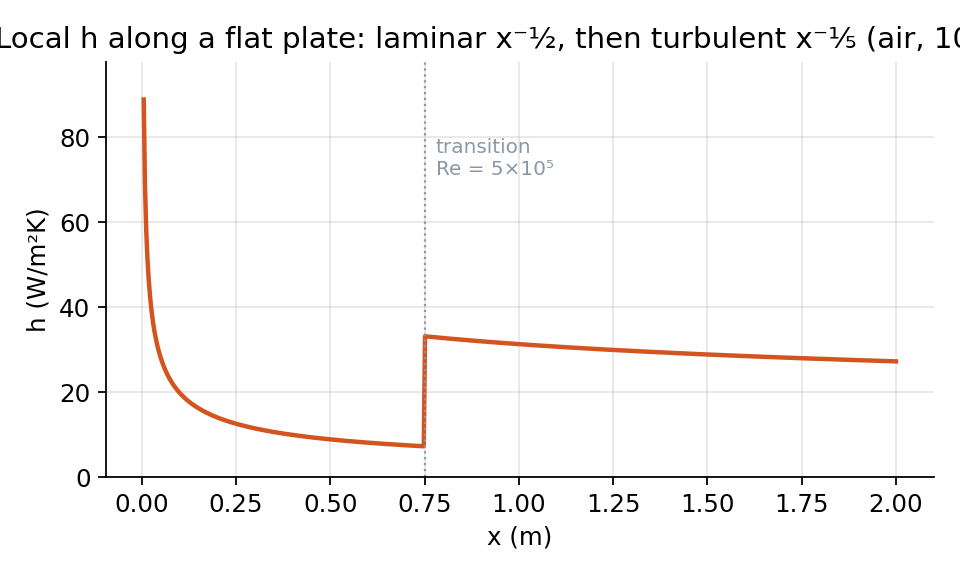
\includegraphics[width=0.35\linewidth]{pics/h_vs_x.png}
    \caption{Axial variation of the convection heat transfer
coefficient for flow in a tube.}
\end{figure}
%%%%%%%%%%%%%%%%%%%%%%%%%%%%%%%%%%%%%%%%%%%%%%%%%%%%%%%%%%%%%
\subsection*{Energy Analysis of Internal Flow}
\addcontentsline{toc}{subsection}{Energy Analysis of Internal Flow}
%%%%%%%%%%%%%%%%%%%%%%%%%%%%%%%%%%%%%%%%%%%%%%%%%%%%%%%%%%%%%
\subsubsection*{Key Assumptions}
\addcontentsline{toc}{subsubsection}{Key Assumptions}
%%%%%%%%%%%%%%%%%%%%%%%%%%%%%%%%%%%%%%%%%%%%%%%%%%%%%%%%%%%%%
For most internal flow analyses, we make the following assumptions:
%
\begin{enumerate}
    \item \textbf{Neglect axial conduction} - Justified by comparing advection to axial conduction:
   \[
   \frac{\text{advection}}{\text{axial conduction}} = \frac{\rho c_p u_m T_m}{k\frac{dT_m}{dx}} \gg 1
   \]
   For typical water flow at 1 m/s with temperature change of 100°C over 1 m:
   \[
   \frac{\text{advection}}{\text{axial conduction}} \approx \frac{1000 \times 4000 \times 1 \times 50}{0.6 \times 100} \approx 3.3 \times 10^6
   \]
   This means axial conduction contributes less than one part per million to the heat transfer.
    %
    \item \textbf{Incompressible flow} - Valid for liquids and gases at low speeds
    %
    \item \textbf{Constant properties} - Can be evaluated at the bulk temperature or film temperature
    %
    \item \textbf{No internal heat generation} - Unless specifically considered in the problem
\end{enumerate}
%
%%%%%%%%%%%%%%%%%%%%%%%%%%%%%%%%%%%%%%%%%%%%%%%%%%%%%%%%%%
% \subsubsection*{Energy Balance for Internal Flow}
% \addcontentsline{toc}{subsubsection}{Energy Balance for Internal Flow}
% %%%%%%%%%%%%%%%%%%%%%%%%%%%%%%%%%%%%%%%%%%%%%%%%%%%%%%%%%%
% For a differential control volume in a pipe with these assumptions, the energy balance is:
% \[
% \dot{m}c_p dT_m = q_s'' P dx
% \]

% Where:
% \begin{itemize}
%     \item $\dot{m}$ is the mass flow rate
%     \item $c_p$ is the specific heat
%     \item $dT_m$ is the change in bulk temperature
%     \item $q_s''$ is the surface heat flux
%     \item $P$ is the perimeter of the pipe ($P = \pi D$ for a circular pipe)
%     \item $dx$ is the differential length
% \end{itemize}

% This can be rewritten using the heat transfer coefficient:
% \[
% \dot{m}c_p dT_m = h[T_s(x) - T_m(x)]P dx
% \]
% %%%%%%%%%%%%%%%%%%%%%%%%%%%%%%%%%%%%%%%%%%%%%%%%%%%%%%%%%%%%%
% \subsection*{Constant Surface Temperature Case}
% \addcontentsline{toc}{subsection}{Constant Surface Temperature Case}
% %%%%%%%%%%%%%%%%%%%%%%%%%%%%%%%%%%%%%%%%%%%%%%%%%%%%%%%%%%%%%
% For constant surface temperature ($T_s = \text{constant}$), the energy balance can be integrated:
% \[
% \frac{T_s - T_m(x)}{T_s - T_i} = \exp\left(-\frac{hP}{\dot{m}c_p}x\right) = \exp\left(-\frac{4hx}{Gc_pD}\right)
% \]

% Where:
% \begin{itemize}
%     \item $T_i$ is the inlet temperature
%     \item $G = \frac{\dot{m}}{\pi D^2/4}$ is the mass flux
% \end{itemize}

% The bulk temperature approaches the surface temperature exponentially:
% \[
% T_m(x) = T_s - (T_s - T_i)e^{-x/x_c}
% \]

% Where $x_c = \frac{\dot{m}c_p}{hP}$ is the characteristic length.

% The total heat transfer rate from inlet to position $x$ is:
% \[
% q = \dot{m}c_p[T_m(x) - T_i] = \dot{m}c_p(T_s - T_i)(1 - e^{-x/x_c})
% \]
% %%%%%%%%%%%%%%%%%%%%%%%%%%%%%%%%%%%%%%%%%%%%%%%%%%%%%%%%%%%%%
% \subsection*{Constant Heat Flux Case}
% \addcontentsline{toc}{subsection}{Constant Heat Flux Case}
% %%%%%%%%%%%%%%%%%%%%%%%%%%%%%%%%%%%%%%%%%%%%%%%%%%%%%%%%%%%%%
% For constant heat flux ($q_s'' = \text{constant}$), the energy balance gives:
% \[
% \frac{dT_m}{dx} = \frac{q_s''P}{\dot{m}c_p} = \text{constant}
% \]

% Thus, the bulk temperature increases linearly with distance:
% \[
% T_m(x) = T_i + \frac{q_s''P}{\dot{m}c_p}x
% \]

% The surface temperature can be calculated from:
% \[
% T_s(x) = T_m(x) + \frac{q_s''}{h(x)}
% \]

% In the thermally fully developed region where $h$ is constant, the surface temperature also increases linearly with the same slope as the bulk temperature.
% %%%%%%%%%%%%%%%%%%%%%%%%%%%%%%%%%%%%%%%%%%%%%%%%%%%%%%%%%%%%%
% \subsection*{Nusselt Number for Internal Flow}
% \addcontentsline{toc}{subsection}{Nusselt Number for Internal Flow}
% %%%%%%%%%%%%%%%%%%%%%%%%%%%%%%%%%%%%%%%%%%%%%%%%%%%%%%%%%%%%%
% The Nusselt number for internal flow is defined as:
% \[
% \text{Nu}_D = \frac{hD}{k}
% \]

% For fully developed laminar flow:
% \begin{enumerate}
%     \item Constant surface temperature:
%     \[
%         \text{Nu}_D = 3.66
%     \]
%     %
%     \item Constant heat flux:
%     \[
%         \text{Nu}_D = 4.36
%     \]
% \end{enumerate}
% %
% For turbulent flow ($\text{Re}_D > 2300$), the Dittus-Boelter equation is commonly used:
% \[
%     \text{Nu}_D = 0.023\text{Re}_D^{0.8}\text{Pr}^n
% \]

% Where:
% \begin{itemize}
%     \item $n = 0.4$ for heating of the fluid ($T_s > T_m$)
%     \item $n = 0.3$ for cooling of the fluid ($T_s < T_m$)
% \end{itemize}

% For the entrance region, higher Nusselt numbers occur due to developing boundary layers. Correlations exist for both laminar and turbulent entrance regions.